\begin{song}{title=\predtitle \centering Slunečný hrob \\\large Blue Effect  \vspace*{-0.0cm}}  %% sem se napíše jméno songu a autor

\velky

\begin{centerjustified}

\ssloka{Rec:} Usínám a chtěl bych se vrátit o nějakej ten rok zpátky,

bejt zase malým klukem, kterej si rád hraje a který je s tebou.

\sloka
^{\z E}Zdá se ^{F#mi}mi, ^{Asmi}je to ^{\z F#mi}moc let,

já byl kluk,  kterej chtěl

znáti svět,  s tebou jsem si hrál.

\sloka
Vrátím se a chtěl bych rád

být s tebou, zavzpomínat,

^{E}mám tu ^{\z F#mi}teď ^{Asmi}ale ^{\z F#mi}zprávu ^{\z E}zlou. ^{    E   E7  E7}

\refren
^{C#mi \z}Su - ^{\z C#mi}chá ^{\z Esmi}hlína ^{A \z}ta - ^{Asmi}dy, ^{F#mi}

^{C#mi \z}bez ^{C#mi \z}kví - ^{Esmi \z}tí, ^{A}bez vo - ^{Asmi}dy, ^{F#mi}

^{Asmi}já na ni ^{F#mi \z}poklekám,

^{Asmi \z}vzpomínkou pocta ^{H7 \z}se vzdává.

\sloka
Loučím se a něco však

tam zůstalo z těch našich dnů,

já teď vím, věrný zůstanu.


\ssloka{Rec:} Nemohu spát, probouzím se a zase se nemohu ubránit myšlence,

vrátit se o nějakej ten rok zpátky, bejt zase malým klukem,

který si rád hraje, který je s tebou.


\end{centerjustified}

\centering
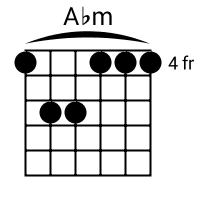
\includegraphics[width=3cm]{../Akordy/asmi.png}
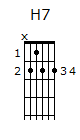
\includegraphics[width=3cm]{../Akordy/h7.png}
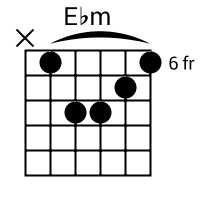
\includegraphics[width=3cm]{../Akordy/esmi.png}


%\centering
%\normalsize Pozn.: závorky značí kánon.

\setcounter{Slokočet}{0}
\end{song}


